\documentclass[11]{article}

\usepackage{graphicx}
\usepackage{hyperref}
\usepackage{subcaption}
\usepackage{amsmath}
\usepackage[
    backend=bibtex,
%    isbn=false,
%    url=false,
%    doi=false,
%    eprint=false,
%    hyperref=false,
%    backref=false,
%    firstinits=false,
]{biblatex}
\bibliography{references}

\hypersetup{colorlinks,urlcolor=blue}
\let \shorttitle \textbf
\begin{document}

\section{Introduction}
Tool use is one of the human abilities that uniquely distinguishes man from other species. 
We refer to tools as hand held devices used in making changes to the surrounding environment. 
Cases of tool use have been reported in other species, but never to the magnitude engaged by humans \cite{boysen1999,harrington2009,lefebvre2004}. 
As a defining attribute of human cognition, we wish to lay the foundations for a computational model of the reasoning processes involved.

\subsection{The four constraints theory}
Our model stems from the architectural framework defined by the four constraints theory (4CT) \cite{osiurak2014a}.
4CT characterises tool use for healthy individual's behaviour.
Its theoretical basis lie however on the empirical investigations of aprxia and the cognitive impairments caused.
Apraxia is a neurological disorder impairing a person's ability to plan and execute sequences of movements.
The term covers a multitude of symptoms and levels of severity (e.g. dyspraxia, ideomotor aparaxia, apraxia of speech) .
The underlying cause for these disorders is physical damage to the left hemisphere of the brain\cite{osiurak2013}.

\begin{figure}[h]
  \centering
  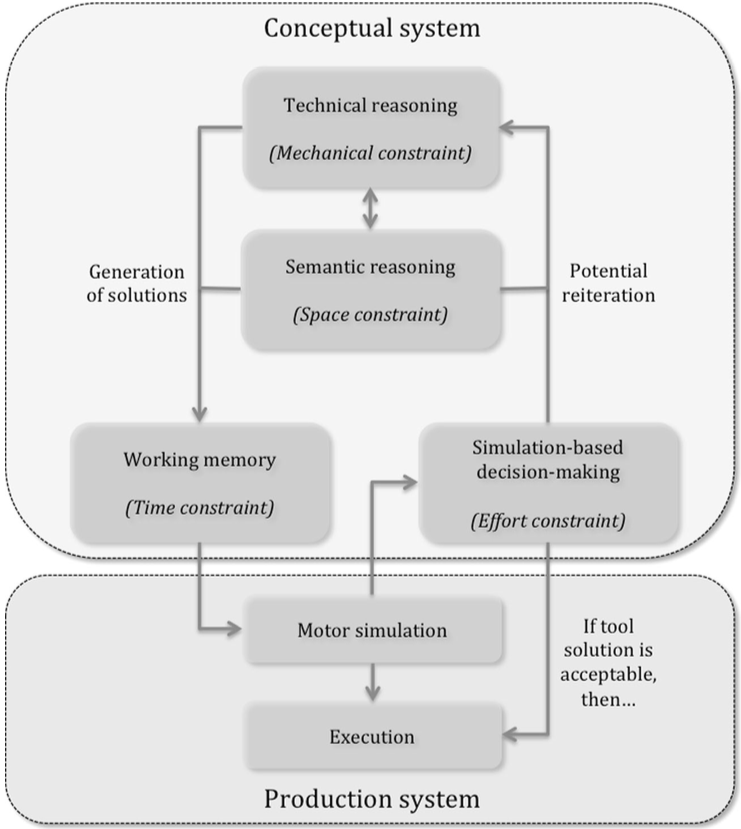
\includegraphics[width=.9\textwidth]{./figures/4CTArchitecture.png}
  \caption{4CT architecture reprinted from \cite{osiurak2014a}}
  \label{fig:4CTArchitecture}
\end{figure}      

4CT structures tool use into a conceptual system and a production system (fig. \ref{fig:4CTArchitecture}).
The theory mostly focuses on the conceptual level which encapsulates cognitive reasoning.
Task execution is handled by the production system which dictates motor movement.   
Due to the distinction, 4CT's conceptual system is a suitable candidate for a computational model concentrated on reasoning.

%-----------
% More paragraphs needed to explain why 4CT is desired over other theories
%-----------

The theory characterises tool use situations as problem solving tasks requiring strong cognitive abilities. 
The four constraints of \emph{mechanics, space, time,} and \emph{effort} are the dimensions within which problems are defined.
Aiding problem solving are four cognitive processes: \emph{technical reasoning, semantic reasoning, working memory,} and \emph{simulation based decision making} (fig. \ref{fig:4CTArchitecture}).  
Even simple scenarios of slicing bread requires reasoning about the knife's sharpness,length, hardness, and the movements necessary to manifest the mechanical effect of cutting. 

Problem solving becomes more apparent in the absence of familiar tools, when subjects are required to repurpose tools or fashion new ones.
A distinction is made between novel tool use and familiar use. 
Semantic reasoning refers to situations when subjects are accustomed with a tool's common use. 
For example a knife is used for cutting bread. 
The association is made on prior experience without considering the knife's physical properties.  
In novel cases however, technical reasoning is the inference of how object properties can solve problems.
In the absence of a bread knife a saw would be a better cutting device than a spreading knife. 
Technical reasoning is a more general process for solving problem but is more cognitively involved.  

The effort constraint and simulation based decision making refer to tool use energy cost. 
A simple rule of survival is that actions should require less energy than the rewards gained \cite{proffitt2006}.
Perceived effort would explain user's preference for one tool use method over another. 
Even when multiple tools are available, differences in their physical properties can lead to differences in effort that further dictate choice. 

Working memory is required in the context where multiple steps must be fulfilled to achieve a goal. 
It describes a subject's ability to split activities into sub-goals and hold them in memory. 
Complex tasks such as fixing a radio would involve multiple steps and tool selection. 
However, such complex objectives are beyond the scope of this project.

A computational model should initially solve simple tool-use problems before complex ones.
Our focus is therefore on single step tool and object interaction involving generic situations.
These situations would be best solved through technical reasoning for its general problem solving abilities. 
However, beyond simple attributes such as object length,sharpness,abrasiveness, 4CT is not able to explain human decision-making.
Crucial factors of forces and geometric constraints are simply abstracted as mechanical knowledge. 
A computational model would therefore have to elaborate these items before fitting into the larger 4CT framework. 
The topic of this paper is solving geometric constraints through spatial reasoning in order to achieve simple tool-object interaction.  

\section{Experimental Setup}

The experimental setup was devised by Dietmar Heinke and Fran\c{c}ois Osiurak (the author of 4CT). 
It is intended for use in both a computational model and to investigate human reasoning on tool and object geometries. 
Human trials were run in parallel to this project but do not constitute part of it. 
Nevertheless, this paper will refer to observations of human behaviour, even though data has not yet been published. 

\begin{figure}[!h]
  \centering
  \begin{subfigure}{0.49\textwidth}
    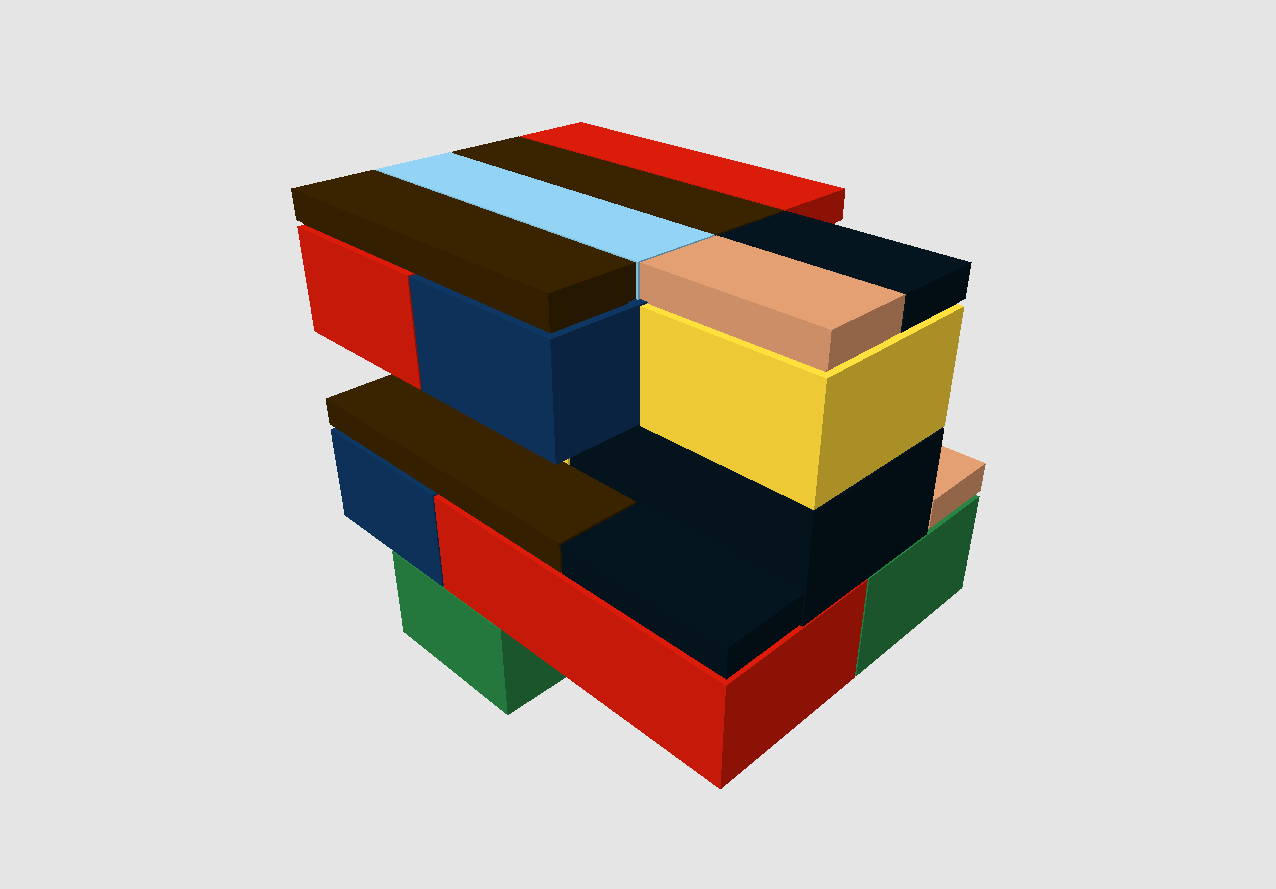
\includegraphics[width=1\linewidth]{./figures/obj51.png}
    \caption{Passive object}
    \label{fig:obj51}
  \end{subfigure}
  \begin{subfigure}{0.49\textwidth}
    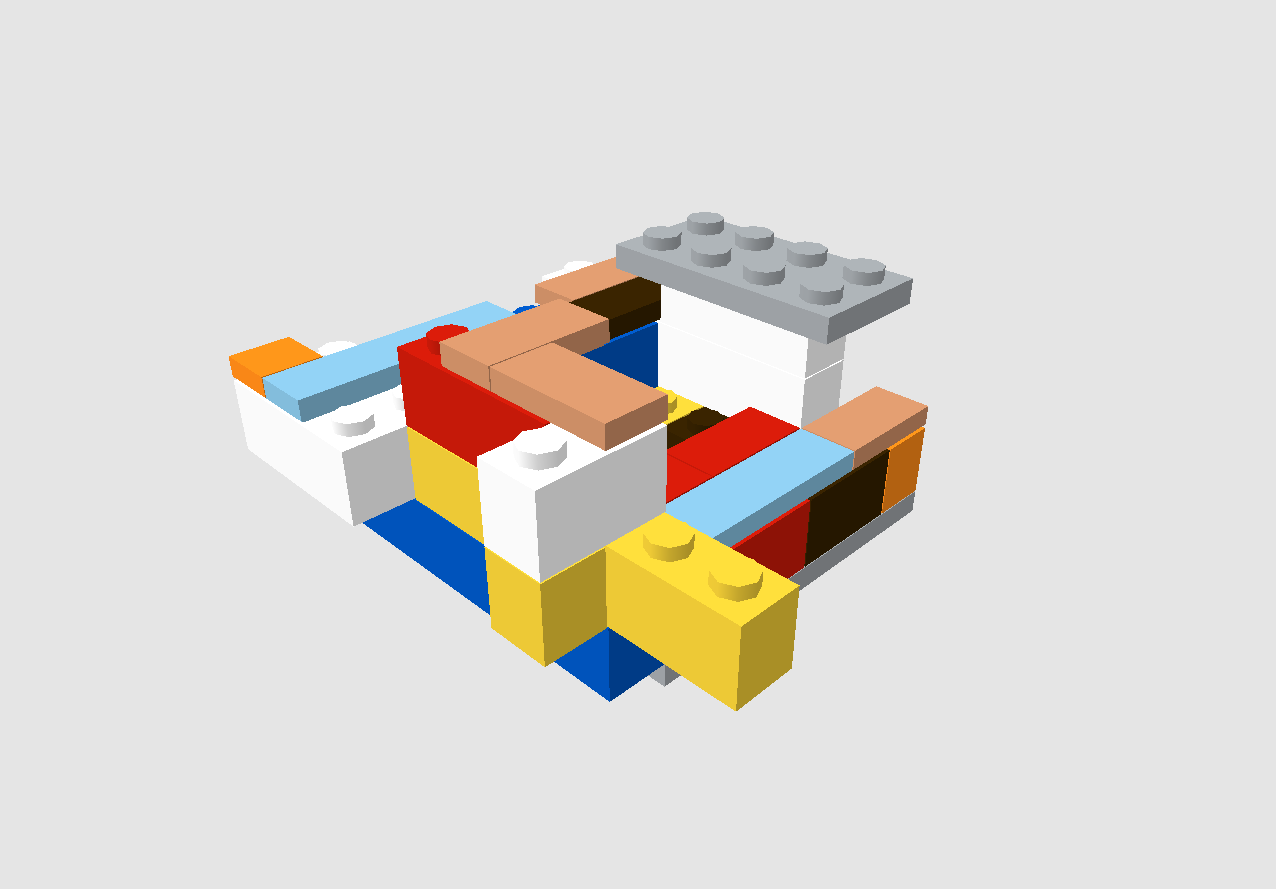
\includegraphics[width=1\linewidth]{./figures/obj52.png}
    \caption{Active object}
    \label{fig:obj52}
  \end{subfigure}
  \caption{Pair of novel tool and object models}
\end{figure}

In the experiment, a human subject is presented two novel objects composed out of LEGO blocks.
One object is passive and may not be directly touched (fig. \ref{fig:obj51}).
The second object is active and must be used to lift the passive object to a new location (fig. \ref{fig:obj52}).
The active and passive objects are analogous to a tool and target object respectively.

Because of the unusual geometries, subjects must reason about the spatial fitting of the tool and object, in order to complete their task.    
Formally solving object-tool fitting requires considerations of force closure.
However, a shortcut to computing physical interaction is to consider the use of a physics engine. 
To some extent, it is believed that the human brain computes approximate of Newtonian laws \cite{battaglia2013}. 
Similarly, physics engines do not compute exact friction, closure or gravity laws, but provide realistic dynamic results. 
A computational model for tool use can employ physics engines for one of multiple reasons:
\begin{enumerate}
      \item it can serve as an engine for inference over physical laws   
      \item it can verify solutions of tool-object configurations through simulation
      \item it is analogous to mental simulation (4CT)
\end{enumerate}

\section{Physics Engine Review}
We consider physics engines written in C++ or available to Matlab for our model. 
Preferably these engines should be free or have reduced licensing fees. 
Our experiments require specifically rigid body simulations, as LEGO objects have no joints or moving parts.

In large majority engines are aimed at game development\ref{boeing2007,roennau2013,hummel2012}. 


\printbibliography
\end{document}
